\documentclass[journal]{IEEEtran}
\usepackage{cmap}
\usepackage{amsmath}
\usepackage{amsfonts}
\usepackage{subfigure}
\usepackage[final]{graphicx}
\usepackage{graphics,picture}
\usepackage{mathrsfs}
\usepackage{cases}
\usepackage{bm, comment,color,amssymb}
\usepackage{cite,epstopdf}
\usepackage{algorithm}
\usepackage{algorithmic}
\renewcommand{\thefootnote}{\arabic{footnote}}
\newcommand{\trace}{\mathop{\mathrm{Tr}}}%\trace
\newcommand{\vectorize}{\mathop{\mathrm{vec}}}%\vectorization

\begin{document}
	
\title{Decentralized Blockchain Based Dynamic Spectrum Acquisition for Wireless Downlink Communications}
	
\author{Miao Jiang, Yiqing Li, Qi Zhang, \emph{Member}, \emph{IEEE}, and Jiayin Qin

\thanks{M. Jiang, Y. Li, and Q. Zhang are with the School of Electronics and Information Technology, Sun Yat-sen University, Guangzhou 510006, Guangdong, China (e-mail: jmiao@mail2.sysu.edu.cn, liyiq5@mail2.sysu.edu.cn, zhqi26@mail.sysu.edu.cn). J. Qin is with the School of Electronics and
Information Technology, Sun Yat-sen University, Guangzhou 510006, Guangdong,  China, and also with the Xinhua College, Sun Yat-sen University, Guangzhou 510520, Guangdong, China (e-mail: issqjy@mail.sysu.edu.cn).}
}% <-this % stops a space
	
	
\markboth{}
{Jiang \MakeLowercase{\textit{et al.}}: Decentralized Blockchain Based Dynamic Spectrum Acquisition for Wireless Downlink Communications}
	
\maketitle
\begin{abstract}
Wireless network virtualization is a promising solution to improve the spectrum efficiency. For a wireless downlink communication system with multiple mobile virtual network operators (MVNOs), we propose a decentralized blockchain based dynamic spectrum acquisition scheme. Our proposed scheme aims to minimize the sum transmit power at all MVNOs while satisfying the average data transmission rate thresholds. For each MVNO,
the required wireless spectrum to provide customized services to the mobile users (MUs) is predicted using the half-range Gauss-Hermite quadrature. Based on the predicted values, all the MVNOs carry out a blockchain-based distributed alternative direction method of multipliers to obtain the global optimal solution to the aforementioned sum transmit power minimization problem. To examine the effectiveness of our proposed scheme, with known system parameters, we also theoretically derive the semi-closed-form solution to the actual required sum transmit power minimization problem subject to data transmission rate constraints. Simulation results illustrate that our proposed dynamic spectrum acquisition scheme achieves almost the same minimum sum power as the non-causal scheme which assumes the number of active MUs in all cells and all the channels are known non-causally for the optimal dynamic spectrum allocation.
\end{abstract}
\begin{IEEEkeywords}
Alternating direction method of multipliers (ADMM), blockchain, dynamic spectrum acquisition, wireless network virtualization.
\end{IEEEkeywords}
\IEEEpeerreviewmaketitle
	
\section{Introduction}

With the popularity of various smart phones, an exponential traffic growth is generated by wireless applications in next generation 5G networks and beyond \cite{NPanwar,DingZ14,LiY17,LiY18}. To cope with the dramatic traffic growth, network densification is expected to increase by 1000 times ranging from macrocells to femtocells \cite{AYDing}. Thus, a serious spectrum shortage problem should be properly addressed. To solve the spectrum shortage problem, either we release more licensed bandwidth for next generation 5G networks and beyond, or we improve the spectrum efficiency by employing the efficient spectrum management schemes.

To improve the spectrum efficiency, wireless network virtualization is a promising solution \cite{CLiang,LZhao,3GPP}. Wireless network virtualization is able to facilitate multiple network operators to share common resources, e.g., licensed spectrum. The virtualized wireless networks (VWNs) commonly consist of multiple mobile network operators (MNOs) and multiple mobile virtual network operators (MVNOs) \cite{RKokku}. The MNO owns the physical cellular infrastructure and radio resources, it executes the virtualization by leasing the isolated virtualized network resources to the MVNO. The MVNO leases the resources from the MNO and then assigns the resources to the MUs. The spectrum resources which belong to one or more MNOs are virtualized and spitted into slices. The MVNO utilizes the slices leased from MNOs depending on the quality-of-service (QoS) of MUs. Recently, wireless network virtualization had attracted an increasing attention from the research community \cite{XCostaPerez,MIKamel,MKalil,YXZhang}. In \cite{XCostaPerez}, an active sharing of physical infrastructure and the spectrum was proposed, where MNOs share the network resources and provide wholesale access to MVNOs, allowing them to provide voice and data services using part of the available resources. The work in \cite{MIKamel} introduced a novel scheme for slicing and scheduling for VWNs by developing an efficient resource allocation scheme. In \cite{MKalil}, an efficient low-complexity scheme was put forward to virtualize the wireless resource blocks and share them between MUs of multiple MNOs. The scheme aims to maximize the throughput while maintaining access proportional fairness among MUs as well as MNOs. In \cite{YXZhang}, a two-stage spectrum leasing problem with the goal of maximizing the average profit of a VMNO was investigated.

Aforementioned dynamic spectrum allocation schemes in VWNs improve the spectrum efficiency in a centralized manner which requires a central node.
If the central node is under cyberattack, all the MVNOs are vulnerable. In addition, if the MVNOs belong to different MNOs, the information exchange among different nodes should be as less as possible. Furthermore, the management overhead increases with the increase of the number of MVNOs which causes that the wireless communication system is not scalable. Therefore, in this paper, we propose a decentralized blockchain based dynamic spectrum acquisition scheme.

Blockchain, which was invented by Satoshi Nakamoto in 2008, is an emerging technology to build consensus between disparate individuals \cite{SNakamoto}. The intuition is to solve the double-spending problem in the cryptocurrency bitcoin without the use of a trusted central utility. Blockchain consists of lists of blocks which are linked by the hash algorithm. Each block includes collections of signatured transactions. A new block can be appended to the end of the current blockchain after solving a proof-of-work (PoW) puzzle which is to find a number whose hash value is less than the current target. PoW can create distributed consensus between all participants and solve the double-spending problem. The data on blockchain is shared and saved by all participants on peer-to-peer networks. All participants have right to access but cannot tamper the data on blockchain. The pillars of blockchain are state-of-the-art cryptography and PoW based distributed consensus mechanism. This kind of system may introduce some computational cost but can provide decentrality, security, transparency and robustness. The blockchain technologies have been extensively used in many areas \cite{KGai,PKSharma,ZXiong,DBRawat,Munsing,KKotobi}.

In this paper, we propose a decentralized blockchain based dynamic spectrum acquisition scheme for a wireless downlink communication system with multiple MVNOs. With wireless network virtualization operation, the whole communication processes are divided into multiple periods, each measured in minutes. At the beginning of each period, MVNOs should predict the required wireless spectrum to provide customized services to the MUs in their respective service cells. Based on the predicted values, MVNOs acquire wireless spectrum by our proposed decentralized blockchain based dynamic spectrum acquisition scheme. Our proposed scheme aims to minimize the sum transmit power at all MVNOs while satisfying the average data transmission rate thresholds. We propose to employ the half-range Gauss-Hermite quadrature (HR-GHQ) to simplify the optimization problem. Then, we propose a blockchain-based distributed alternative direction method of multipliers (ADMM) to obtain the global optimal solution to aforementioned sum transmit power minimization problem.

To fairly compare the performance of our proposed scheme with the fixed spectrum allocation scheme and other schemes, with known system parameters, we propose to investigate the actual required minimum sum transmit power of all MVNOs subject to that the data transmission rate thresholds for all MUs in all cells are satisfied. We theoretically derive semi-closed-form expressions for the optimal power and spectrum allocation for each MVNO.

The remainder of the paper is organized as follows. The system model and dynamic spectrum acquisition optimization problem formulation are described in Section II and Section III, respectively. We propose the blockchain based distributed ADMM algorithm for dynamic spectrum acquisition in Section IV. With known system parameters, the optimal power and spectrum allocation is theoretically derived in Section V. Section VI provides simulation results to validate the effectiveness of our proposed scheme. Section VII concludes this paper.

\emph{Notations}: Boldface lowercase letters denote vectors. $\left(\cdot\right)^T$ denotes the transpose operation. $\left\|\cdot \right\|_1$ and $\left\|\cdot \right\|_2$ represent the $l_1$ and $l_2$ norm of a vector, respectively.

\section{System Model}

Consider a wireless downlink communication system with $M$ MVNOs. Each MVNO serves the MUs in a cell. The $m$-th transmission cell, $m\in\mathcal{M}=\{1,2,\cdots,M\}$, is assumed to be a fixed circular region, denoted as  $\mathcal{D}_m\in \mathbb{R}^2$, whose radius is denoted as $r_m$. The $m$-th MVNO is located at the cell center.

With wireless network virtualization operation, the whole communication processes are divided into multiple periods, each measured in minutes. At the beginning of each period, MVNOs should predict the required wireless spectrum to provide customized services to the MUs in their respective service cells. Based on the predicted values, MVNOs acquire wireless spectrum. Denote the bandwidth of wireless spectrum acquired by the $m$-th MVNO as $w_m$, for $m\in\mathcal{M}$. We have
\begin{align}\label{q1}
\sum_{m=1}^{M} w_m \leq W
\end{align}
where $W$ denotes the total available bandwidth.

To predict the required wireless spectrum in a period, the active MUs in the $m$-th cell are modeled as a Poisson point process (PPP) with density $\lambda_m$. Suppose that transmitted signals are affected by both large-scale path loss and small-scale flat Rayleigh fading. Thus, the channel between the $n$-th MU and its associated $m$-th MVNO is denoted by
\begin{equation}
h_{mn}=\frac{g_{mn}}{\sqrt{1+L_{mn}^\alpha}}
\end{equation}
where $L_{mn}$ denotes the distance between the $m$-th MVNO and the $n$-th MU in the $m$-th cell, $\alpha$ denotes the path-loss decay factor, and $g_{mn}$ denotes a complex Gaussian random variable with zero mean and unit variance. The instantaneous data rate for the $n$-th MU in the $m$-th MVNO is given by
\begin{align}
R_{mn} = b_{mn}\log_2\left(1+\frac{q_{mn}\left|h_{mn}\right|^2 }{\Gamma b_{mn}\sigma_0^2}\right)
\end{align}
where $b_{mn}$ and $q_{mn}$ denote the bandwidth and power of the $n$-th MU allocated by the $m$-th MVNO, respectively, $\Gamma$ denotes the signal-to-noise ratio (SNR) gap to the information theoretical channel capacity owing to the non-ideal coding and modulation in practice \cite{JGDForney}, and $\sigma_0^2$ denotes the power spectral density of additive white Gaussian noise at all MUs.


\section{Dynamic Spectrum Acquisition Optimization Problem Formulation}

For the required wireless spectrum prediction, since we have no information on the channels, $h_{mn}$, we employ the uniform bandwidth allocation and power allocation for the MUs in each cell. Thus, in the $m$-th cell,
\begin{equation}
b_{mn} = \frac{w_m}{N_m} \mbox{ and }q_{mn}=\frac{p_m}{N_m}
\end{equation}
where $N_m$ denotes the number of active MUs in the $m$-th cell and $p_m$ denotes the total transmission power budget at the $m$-th MVNO. Since the active MUs in the $m$-th cell are modeled as a PPP with density $\lambda_m$, the average number of MUs in the $m$-th cell is
\begin{equation}
\mathbb{E}[N_m]=\Lambda_m=\pi r_m^2 \lambda_m.
\end{equation}
Accordingly, the expected data transmission rate of the $j$-th MU in the $i$-th cell is expressed as
\begin{align}
\mathbb{E}\left[{R}_{mn}\right] = \sum_{N_m=1}^{\infty}\frac{\Omega}{N_m}\mbox{Pr}[N_m]
\end{align}
where
\begin{align}
\label{q5}\Omega&=\int_{0}^{\infty} w_m\log_2\left(1 + \frac{p_m x}{w_m \sigma^2}\right) f_{\left|h_{ij} \right|^2} \left(x\right)dx,\\
\mbox{Pr}[N_m]&=\frac{(\Lambda_m)^{N_m}}{N_m!}\exp\left(-\Lambda_m\right).
\end{align}
In \eqref{q5}, $\sigma^2=\Gamma \sigma_0^2$ and $f_{\left|h_{ij} \right|^2} \left(x\right)$ is the probability density function (PDF) of the random variable $\left|h_{ij} \right|^2$. According to \cite{MAbramowitz}, we have
\begin{align}
\sum_{N_m=1}^{\infty}\frac{1}{N_m}\mbox{Pr}[N_m]=\phi_m
\end{align}
where
\begin{align}\label{q6}
\phi_m= \left(\mbox{Ei}\left(\Lambda_m\right) - \ln\left(\Lambda_m\right)- C\right)\exp\left(-\Lambda_m\right).
\end{align}
In \eqref{q6}, $\mbox{Ei}\left(x\right)$ is the exponential integral function whose series expansion is \cite[5.1.10]{MAbramowitz}
\begin{equation}
\mbox{Ei}\left(x\right) =\sum\limits_{n = 1}^{\infty}\frac{x^n}{n\cdot n!}+\ln x+C
\end{equation}
and $C$ denotes the Euler-Mascheroni constant.

Denote the average data transmission rate threshold for each MU in the $m$-th cell as $\bar{R}_m$, for $m\in\mathcal{M}$. Note that with limited $w_m$, to ensure that
\begin{align}\label{q7}
\mathbb{E}\left[{R}_{mn}\right]\geq \bar{R}_m,
\end{align}
we may increase $p_m$. Thus, to reasonably allocate wireless spectrum among different MVNOs, we should minimize the sum transmit power at all MVNOs while satisfying the average data transmission rate thresholds, which is
formulated as
\begin{align}\label{q8}
\min_{\mathbf{p}, \mathbf{w}}\ & \sum\limits_{m=1}^{M} p_m \nonumber\\
\mbox{s.t.}\ &\eqref{q1},\ \eqref{q7},\ p_m \geq 0,\ w_m \geq 0,\ \forall\ m\in\mathcal{M}
\end{align}
where  $\mathbf{p} = \left[p_1, p_2, \cdots, p_M\right]^T$ and $\mathbf{w} = \left[w_1, w_2, \cdots, w_M\right]^T$. To proceed, we will first introduce the following proposition.

\textit{Proposition 1}: The cumulative distribution function (CDF) of $\left|h_{mn} \right|^2$ is
\begin{equation}\label{q9}
F_{\left|h_{mn} \right|^2}\left(x\right) = 1 - \Psi\left(\frac{2}{\alpha}, 1 + \frac{2}{\alpha}, - x r_m^{\alpha}\right)e^{-x}
\end{equation}
where $\Psi\left(a,b,z\right)$ denotes the Kummer's function \cite{MAbramowitz}.

\textit{Proof}: See Appendix A.  $\hfill\blacksquare$

Using Proposition 1, by taking the first-order derivative with respect to $x$, $f_{\left|h_{mn} \right|^2} \left(x\right)$ is
\begin{align}
f_{\left|h_{mn} \right|^2} \left(x\right)=&\Psi\left(\frac{2}{\alpha}, 1 + \frac{2}{\alpha}, -xr_m^{\alpha}\right)e^{-x} \nonumber \\&-\frac{d \Psi\left(\frac{2}{\alpha}, 1 + \frac{2}{\alpha}, -x r_m^{\alpha}\right)}{d x} e^{-x}.
\end{align}
From \cite[13.4.8]{MAbramowitz}, we know
\begin{equation}
\frac{d \Psi\left(s, t, y\right)}{dy} = \frac{s}{t}\Psi\left(s+1, t+1, y\right).
\end{equation}
Thus, we have
\begin{align}\label{q12}
f_{\left|h_{mn} \right|^2} \left(x\right)=e^{-x}\kappa\left(x\right)
\end{align}
where
\begin{align}
\kappa\left(x\right) =& \Psi\left(\frac{2}{\alpha}, 1 + \frac{2}{\alpha}, -xr_m^{\alpha}\right)\nonumber \\ & +\frac{2r_m^{\alpha}}{2+\alpha} \Psi\left(1 + \frac{2}{\alpha}, 2+ \frac{2}{\alpha}, -xr_m^{\alpha}\right).
\end{align}
Substituting \eqref{q12} into \eqref{q7}, we obtain
\begin{equation}\label{q14}
\xi\geq \bar{R}_m
\end{equation}
where
\begin{equation}
\xi=\phi_m\int_{0}^{\infty} w_m\log_2\left(1+\frac{p_m x}{w_m \sigma^2}\right) e^{-x}\kappa\left(x\right) dx.
\end{equation}
It is noted that on the left-hand side of \eqref{q14}, the integral result $\xi$ is difficult to obtain. Furthermore, when the integrand has a non-negligible tail, even the numerical integration is complicated and time-consuming. In this paper, we propose to apply the half-range Gauss-Hermite quadrature (HR-GHQ) to approximate the integral on the left-hand side of \eqref{q14} with high accuracy \cite{JSBall,NMSteen}.

Based on \cite{NMSteen}, a $K$-point HR-GHQ can be written as
\begin{align} \label{q16}
\int_{0}^{\infty}e^{-t^2}\zeta\left(t\right)dt\approx\sum\limits_{k = 1}^{K} a_k \zeta\left(t_k\right)
\end{align}
where both the weights $\{a_k\}_{k = 1}^K$ and abscissas $\{t_k\}_{k = 1}^K$ are real numbers. By letting $x=t^2$, we have
\begin{align} \label{q17}
\xi=\phi_m\int_{0}^{\infty}2w_mt\log_2\left(1 + \frac{p_mt^2}{w_m\sigma^2}\right)e^{-t^2}\kappa\left(t^2\right)dt.
\end{align}
Applying the $K$-point HR-GHQ, we obtain
\begin{align}\label{q18}
\xi\approx\sum\limits_{k= 1}^{K} w_m \eta_{mk}\log_2\left(1 + \frac{p_mt_{mk}^2}{w_m\sigma^2}\right)
\end{align}
where $\eta_{mk}=2\phi_m a_{mk}t_{mk}\kappa\left(t_{mk}^2\right)$, and both the weights $\{a_{mk}\}$ and abscissas $\{t_{mk}\}$ are real numbers.

Substituting \eqref{q18} into problem \eqref{q8}, we have the following optimization problem
\begin{align}\label{q19}
\min_{\mathbf{p}, \mathbf{w}}\ & \sum\limits_{m=1}^{M} p_m \nonumber\\
\mbox{s.t.}\ &\sum\limits_{k= 1}^{K}w_m \eta_{mk}\log_2\left(1 + \frac{p_mt_{mk}^2}{w_m\sigma^2}\right)\geq \bar{R}_m,\nonumber\\
&\eqref{q1},\ p_m \geq 0,\ w_m \geq 0,\ \forall\ m\in\mathcal{M}.
\end{align}
Problem \eqref{q19} is convex in terms of optimization variables $\mathbf{p}$ and $\mathbf{w}$. It can be solved efficiently using the interior point method \cite{SBoyd1}. However, to solve problem \eqref{q19} in a centralized manner requires a central node. If the central node is under cyberattack, all the $M$ MVNOs are vulnerable. In addition, since the $M$ MVNOs may belong to different network providers, the information exchanging among different nodes should be as less as possible. Furthermore, the management overhead increases with the increase of $M$ which causes that the wireless downlink communication system is not scalable. To deal with the aforementioned problems, we propose a blockchain-based distributed ADMM algorithm \cite{SBoyd2,EChen} for dynamic spectrum acquisition in this paper.

\section{Blockchain-Based Distributed ADMM Algorithm for Dynamic Spectrum Acquisition}

By introducing auxiliary variable $\mathbf{z} = \left[z_1, z_2, \cdots, z_M\right]^T$, problem \eqref{q19} is reformulated as
\begin{subequations}\label{bq1}
\begin{align}
\label{bq1a}\min_{\mathbf{p}, \mathbf{w}, \mathbf{z}}\ & \sum\limits_{m=1}^{M} p_m \\
\label{bq1b} \mbox{s.t.}\ \ &\sum\limits_{k= 1}^{K}w_m \eta_{mk}\log_2\left(1 + \frac{p_mt_{mk}^2}{w_m\sigma^2}\right)\geq \bar{R}_m,\\
\label{bq1c} &\sum_{m=1}^{M} w_m \leq W,\\
\label{bq1d} &\mathbf{w} - \mathbf{z} = \mathbf{0},\\
\label{bq1e} &\ p_m \geq 0,\ w_m \geq 0,\ z_m \geq 0,\ \forall\ m\in\mathcal{M}.
\end{align}
\end{subequations}
Denote the feasible region of constraint \eqref{bq1c} and $z_m\geq 0$, $\forall\ m\in\mathcal{M}$ as $\mathcal{Z}$, its indicator function is defined as
\begin{equation}\label{bq2}
\mathbb{I}_\mathcal{Z}\left(\mathbf{z}\right) = \left\{ \begin{array}{lcl}
0, &\mbox{if} \ \mathbf{z} \in \mathcal{Z}, \\
\infty, &\mbox{otherwise}.
\end{array}
\right.
\end{equation}
Similarly, denote the feasible region of constraint \eqref{bq1b}, $p_m\geq 0$ and $w_m\geq 0$, $\forall\ m\in\mathcal{M}$ as $\mathcal{C}$, its indicator function can be defined as
\begin{equation}\label{bq3}
\mathbb{I}_\mathcal{C}\left(\mathbf{p},\mathbf{w}\right) = \left\{ \begin{array}{lcl}
0, &\mbox{if} \ \left(\mathbf{p}, \mathbf{w}\right) \in \mathcal{C}, \\
\infty, &\mbox{otherwise}.
\end{array}
\right.
\end{equation}
With \eqref{bq2} and \eqref{bq3}, problem \eqref{bq1} can be rewritten in ADMM form as follows
\begin{subequations}\label{bq4}
\begin{align}\label{bq4a}
\min_{\mathbf{p}, \mathbf{w}, \mathbf{z}}\ & \sum\limits_{m=1}^{M} p_m + \mathbb{I}_\mathcal{Z}\left(\mathbf{z}\right) + \mathbb{I}_\mathcal{C}\left(\mathbf{p},\mathbf{w}\right)\\
\label{bq4b}\mbox{s.t.}\ \ &  \mathbf{w} - \mathbf{z} = \mathbf{0}.
\end{align}
\end{subequations}
Thus, the augmented Lagrangian (using the scaled dual variable) of problem \eqref{bq4} is given by
\begin{align}
\mathcal{L}_\nu\left(\mathbf{p},\mathbf{w}, \mathbf{z},\mathbf{u}\right)=& \sum\limits_{m=1}^{M} p_m + \mathbb{I}_\mathcal{Z}\left(\mathbf{z}\right) + \mathbb{I}_\mathcal{C}\left(\mathbf{p},\mathbf{w}\right)\nonumber \\ & +\frac{\nu}{2}\left\|\mathbf{w} - \mathbf{z} + \mathbf{u}\right\|_2^2
\end{align}
where $\mathbf{u} = [u_1, u_2, \cdots, u_N]^T$ is the dual variable for the  constraint \eqref{bq4b} and $\nu>0$ is the penalty parameter. From problem \eqref{bq4}, it is observed that the variables can be split into two groups: $\{\mathbf{p}, \mathbf{w}\}$ and $\mathbf{z}$. Furthermore, the objective function can be separable accordingly. Therefore, the ADMM algorithm can be applied to solve problem \eqref{bq4} by iteratively updating $\mathbf{p}, \mathbf{w}$, $\mathbf{z}$ and $\mathbf{u}$.

In the $(l+1)$-th iteration, given $\{\mathbf{p}^{(l)}, \mathbf{w}^{(l)}, \mathbf{z}^{(l)}, \mathbf{u}^{(l)}\}$ which is optimal in the $l$-th iteration, the optimization variables are updated sequentially as follows.

Step 1: Given $\{\mathbf{z}^{(l)}, \mathbf{u}^{(l)}\}$, we solve the following optimization problem
\begin{align}\label{bq6}
\{\mathbf{p}^{(l+1)}, \mathbf{w}^{(l+1)}\} = \arg \max_{\mathbf{p}, \mathbf{w}} \mathcal{L}_\nu\left(\mathbf{p}, \mathbf{w}, \mathbf{z}^{(l)}, \mathbf{u}^{(l)}\right).
\end{align}
Problem \eqref{bq6} is equivalent to
\begin{align}\label{bq7}
\min_{\mathbf{p}, \mathbf{w}}\ & \sum\limits_{m=1}^{M} p_m + \frac{\nu}{2}\sum\limits_{m=1}^{M}\left(w_m-z_m^{(l)}+u_m^{(l)}\right)^2 \nonumber\\ \mbox{s.t.}\ &  \eqref{bq1b},\ w_m\geq 0,\ p_m\geq 0,\ \forall\ m\in\mathcal{M}.
\end{align}
It is noted that problem \eqref{bq7} can be decomposed into $M$ subproblems. Each subproblem solves
\begin{align}\label{bq8}
\min_{p_m, w_m}\ & p_m+\frac{\nu}{2}\left(w_m-z_m^{(l)}+u_m^{(l)}\right)^2 \nonumber\\
\mbox{s.t.} \ & \sum\limits_{k= 1}^{K}w_m \eta_{mk}\log_2\left(1 + \frac{p_mt_{mk}^2}{w_m\sigma^2}\right)\geq \bar{R}_m,\ \nonumber\\
& w_m\geq 0, p_m\geq 0.
\end{align}
Problem \eqref{bq8} is a convex problem and can be solved efficiently using interior point method \cite{SBoyd1}.

Step 2: Given $\{\mathbf{p}^{(l+1)}, \mathbf{w}^{(l+1)}, \mathbf{u}^{(l)}\}$, we solve the following optimization problem
\begin{align}\label{bq9}
\mathbf{z}^{(l+1)}=\arg\max_{\mathbf{z}} \mathcal{L}_\nu\left(\mathbf{p}^{(l+1)}, \mathbf{w}^{(l+1)}, \mathbf{z}, \mathbf{u}^{(l)}\right).
\end{align}
Problem \eqref{bq9} is equivalent to
\begin{align}\label{bq10}
\min_{\mathbf{z}}\ & \left\|\mathbf{w}^{(l+1)}-\mathbf{z}+\mathbf{u}^{(l)} \right\|_2^2 \\ \mbox{s.t.} \ & \left\|\mathbf{z} \right\|_1 \leq W,\  z_m\geq 0,\ \forall\ m\in\mathcal{M}.
\end{align}
Problem \eqref{bq10} is a convex $\ell_1$ ball projection problem \cite{JDuchi}. Its closed-form solution is obtained as follows.

If $\|\mathbf{w}^{(l+1)}+\mathbf{u}^{(l)}\|_1 > W$, we have
\begin{align} \label{bq11}
z_m^{(l+1)}= \max\left\{w_m^{(l+1)}+u_m^{(l)}-\beta, 0\right\}
\end{align}
where
\begin{align}
\beta&=\frac{1}{\tau}\left(\sum\limits_{m=1}^{\tau} \varphi_m - W\right),\\
\tau&= \max_{1 \leq i \leq M} \left\{ i \left|\varphi_i - \frac{1}{i}\left(\sum\limits_{m=1}^{i} \varphi_m - W\right) > 0 \right. \right\},
\end{align}
and $\bm{\varphi} = \left[\varphi_1, \varphi_2, \cdots, \varphi_M\right]^T$
denotes the vector obtained by sorting $\mathbf{w}^{(l+1)}+\mathbf{u}^{(l)}$ in a descending order.

If $\|\mathbf{w}^{(l+1)}+\mathbf{u}^{(l)}\|_1 \leq W$, we have
\begin{align}
z_m^{(l+1)}=w_m^{(l+1)}+u_m^{(l)}.
\end{align}

Step 3: Given $\{\mathbf{w}^{(l+1)}, \mathbf{z}^{(l+1)}\}$, we solve the following optimization problem
\begin{align}\label{bq13}
\mathbf{u}^{(l+1)}=\arg\max_{\mathbf{u}} \mathcal{L}_\nu\left(\mathbf{p}^{(l+1)}, \mathbf{w}^{(l+1)}, \mathbf{z}^{(l+1)}, \mathbf{u}\right).
\end{align}
The closed-form solution to problem \eqref{bq13} is
\begin{align} \label{q24}
\mathbf{u}^{(l+1)} =\mathbf{w}^{(l+1)} - \mathbf{z}^{(l+1)} + \mathbf{u}^{(l)}.
\end{align}

Thus, the whole blockchain-based distributed ADMM algorithm for dynamic spectrum acquisition is summarized in Algorithm 1.

\begin{algorithm}[h]
\caption{Blockchain-Based Distributed ADMM Algorithm for Dynamic Spectrum Acquisition}
\begin{algorithmic}[1]
\STATE \textbf{Initialize}: $z_m^{(0)}=0$ and $u_m^{(0)}=0$ $\forall$ $m\in\mathcal{M}$; $\nu=0$; $l=0$;
\STATE \textbf{Repeat}: \\
\hspace{0.5cm} \textbf{Local Computation}:\\
\hspace{1.0cm} Get $z_m^{(l)}$ and $u_m^{(l)}$ from blockchain;\\
\hspace{1.0cm} Obtain $p_m^{(l+1)}$ and $w_m^{(l+1)}$ by solving \eqref{bq8}; \\
\hspace{1.0cm} Send $w_m^{(l+1)}$ to ADMM aggregator on blockchain;\\
\hspace{0.5cm} \textbf{Blockchain Computation}:\\
\hspace{1.0cm} Obtain $\mathbf{z}^{(l+1)}$ and $\mathbf{u}^{(l+1)}$; \\
\hspace{0.5cm} $l=l+1$;\\
\textbf{Until} Convergence.\\
\end{algorithmic}
\end{algorithm}

\emph{Remark}: Blockchains provide a method for providing a transparent, trustless platform for data computation. This makes a blockchain the perfect platform for conducting the aggregation step of ADMM, allowing all participants to audit the progress of the algorithm, the accuracy of the solution, and the veracity of their scheduled commitments. Further, ADMM is a natural fit for implementation on a blockchain, as it guarantees
convergence yet has a computationally cheap aggregation step (minimizing the burden of verification) \cite{Munsing}.

\section{Optimal Power and Spectrum Allocation with Known System Parameters}

In this paper, we propose a dynamic spectrum acquisition scheme. To fairly compare the performance of our proposed scheme with the fixed spectrum allocation scheme and other schemes, with known system parameters, we propose to investigate the actual required minimum sum transmit power of $M$ MVNOs subject to that the data transmission rate thresholds for all MUs in $M$ cells are satisfied. With our proposed dynamic spectrum acquisition scheme and other spectrum allocation schemes, the bandwidth of wireless spectrum of the $m$-th MVNO, i.e., $w_m$, is known. Thus, the aforementioned optimization problem is decoupled into $M$ transmit power minimization subproblems. For the transmit power minimization subproblem of the $m$-th MVNO, with known system parameters, we should study the power and spectrum allocation optimization problem among all MUs in the $m$-th cell subject to that the data transmission rate thresholds for all MUs in the $m$-th cell are satisfied.

In the $m$-th cell, when the actual number of MUs, $N_m$, and the channel between the $n$-th MU and its associated $m$-th MVNO, $h_{mn}$, are known for $n\in\mathcal{N}_m=\{1,2,\cdots,N_m\}$, the power and spectrum allocation optimization problem is formulated as
\begin{subequations}\label{cq1}
\begin{align}
\label{cq1a} \min_{\mathbf{q}_m, \mathbf{b}_m}\ & \sum\limits_{n=1}^{N_m} q_{mn} \\
\label{cq1b}\mbox{s.t.} \quad &  \sum\limits_{n=1}^{N_m} b_{mn} \leq w_m,\\ \label{cq1c}&  b_{mn}\log_2\left(1 + \frac{q_{mn}\left|h_{mn}\right|^2}{b_{mn}\sigma^2}\right) \geq \tilde{R}_m,\\
\label{cq1d}& q_{mn} \geq 0,\ b_{mn} \geq 0,\ \forall\ n\in\mathcal{N}_m
\end{align}
\end{subequations}
where $\tilde{R}_m$ denotes the data transmission rate threshold for each
MU in the $m$-th cell, $\mathbf{q}_m=\left[q_{m1}, q_{m2}, \cdots, q_{mN_m}\right]^T$, and $\mathbf{b}_m=\left[b_{m1}, b_{m2}, \cdots, b_{mN_m}\right]^T$. To continue, we need the following proposition.

\textit{Proposition 2}: For problem \eqref{cq1}, the optimal $\mathbf{q}_m$ and $\mathbf{b}_m$ should satisfy that constraint \eqref{cq1c} are all active, i.e.,
\begin{align}
b_{mn}\log_2\left(1 + \frac{q_{mn}\left|h_{mn}\right|^2}{b_{mn}\sigma^2}\right)= \tilde{R}_m,\  \forall \ n\in\mathcal{N}_m
\end{align}

\textit{Proof}: See Appendix B. $\hfill\blacksquare$

From Proposition 2, problem \eqref{cq1} is equivalently written as
\begin{align}\label{cq3}
\min_{\mathbf{b}_{m}}\ & \sum\limits_{n= 1}^{N_m} \frac{b_{mn}\sigma^2}{\left|h_{mn}\right|^2}\left(2^{\frac{\tilde{R}_m}{b_{mn}}} - 1\right) \nonumber \\ \mbox{s.t.} \quad &  \sum\limits_{n=1}^{N_m} b_{mn} \leq w_m,\ b_{mn} \geq 0,\ \forall n\in\mathcal{N}_m.
\end{align}
Problem \eqref{cq3} is convex. In the following proposition, we propose to solve problem using the bisection search.

\textit{Proposition 3}: The closed-form optimal solution to problem \eqref{cq3}, denoted by $b_{mn}^o$, is
\begin{align}\label{cq4}
b_{mn}^o= \frac{\tilde{R}_m\ln2}{1 + \mathcal{W}\left(\frac{\mu^o\left|h_{mn}\right|^2 - \sigma^2}{e\sigma^2}\right)},\ \forall\ n\in\mathcal{N}_m
\end{align}
where $\mathcal{W}\left(x\right)$ denotes the Lambert $\mathcal{W}$ function of $x$ \cite{RMCorless} and $\mu^o>0$ is a constant which satisfies $\sum_{n=1}^{N_m} b_{mn}=w_m$. The value of $\mu^o$ can be found by the bisection search over $\left[\mu_{\min}, \mu_{\max}\right]$ with
\begin{equation}\label{cq5}
\mu_{\min}=\frac{\chi}{\max_n\left|h_{mn}\right|^2} \mbox{ and } \mu_{\max}=\frac{\chi}{\min_n\left|h_{mn}\right|^2}
\end{equation}
where
\begin{equation}
\chi=\sigma^2\left(\frac{N_m\tilde{R}_m\ln2}{w_m} - 1\right)\exp\left(\frac{N_m\tilde{R}_m\ln2}{w_m}\right) + \sigma^2.
\end{equation}

\textit{Proof}: See Appendix C.  $\hfill\blacksquare$

\section{Simulation Results}

In this section, we evaluate the performance of our proposed dynamic spectrum acquisition through simulations. We consider a wireless downlink communication system with $M=6$ MVNOs. Each MVNO serves the MUs in a cell. Since each MVNO uses different wireless spectrum for transmission, there is no co-channel interference. Thus, the overlap of different cells will not cause a problem. We assume that the radii and the corresponding user densities of the $M=6$ cells are $(r_1 = 80\mbox{ m, }\lambda_1 = 1200\mbox{ persons/km}^2)$, $(r_2 = 80\mbox{ m, }\lambda_2 = 800\mbox{ persons/km}^2)$, $(r_3 = 100\mbox{ m, }\lambda_3 = 800\mbox{ persons/km}^2)$, $(r_4 = 100\mbox{ m, }\lambda_4 = 1000\mbox{ persons/km}^2)$, $(r_5 = 120\mbox{ m, }\lambda_5 = 1000\mbox{ persons/km}^2)$, and $(r_6 = 120\mbox{ m, }\lambda_6 = 1200\mbox{ persons/km}^2)$. The total available bandwidth is 100 MHz. The path-loss decay factor is 3.76 \cite{3GPP2}. We assume that $\sigma^2=\Gamma\sigma_0^2=-150.9$ dBm/Hz \cite{3GPP2}. In \eqref{q16}, a $K=500$-point HR-GHQ is employed. If not specified, the average data transmission rate threshold in \eqref{q7} and the data transmission rate threshold in \eqref{cq1} are $\bar{R}_1 =\tilde{R}_1=2$ Mbps, $\bar{R}_2 =\tilde{R}_2=0.5$ Mbps, $\bar{R}_3=\tilde{R}_3=0.5$ Mbps, $\bar{R}_4 =\tilde{R}_4=1$ Mbps, $\bar{R}_5=\tilde{R}_5=1$ Mbps, and $\bar{R}_6 =\tilde{R}_6=2$ Mbps.

In Fig. 1, we show the convergence performance of Algorithm 1. From Fig. 1, it is observed that our proposed Algorithm 1 converges for about 10 iterations. Furthermore, it is found that the more bandwidth
is needed when the average number of MUs in the cell multiplied with the average data transmission rate threshold, $\mathbb{E}[N_m]\bar{R}_m$, is large.

\begin{figure}
\centering
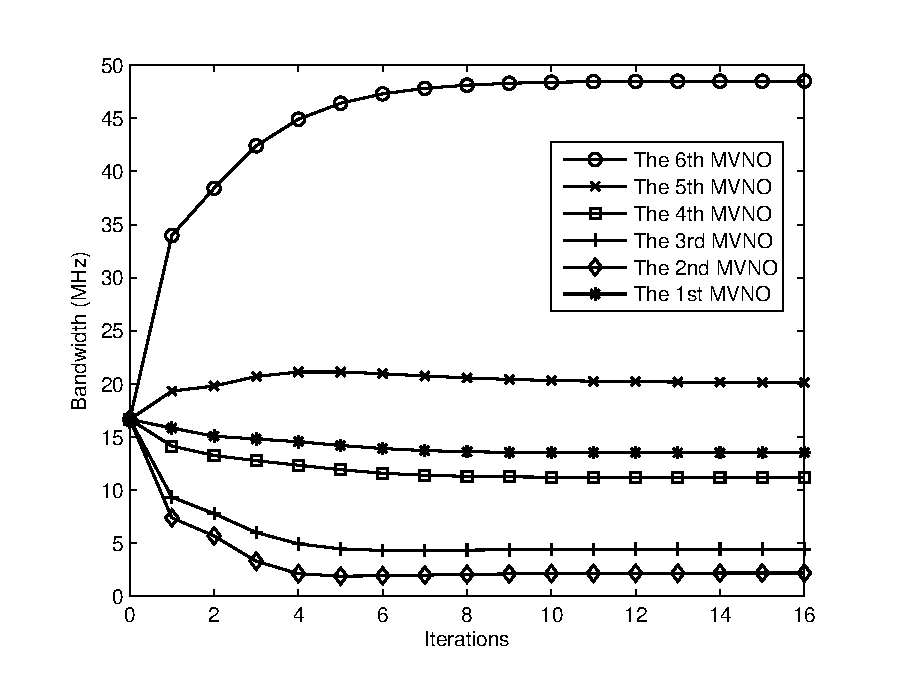
\includegraphics[width=3.6in]{fig1.eps}
\caption{Bandwidth versus iterations; the convergence performance of Algorithm 1.}
\end{figure}

In Fig. 2, we present the minimum sum power comparison of different schemes for different values of the average data transmission rate threshold in the 6-th cell, $\bar{R}_6$. In the legend, ``DSA" denotes our proposed dynamic spectrum acquisition scheme. ``Uniform" denotes that the total available bandwidth is uniformly allocated to $M=6$ MVNOs. ``Proportional" denotes that the total available bandwidth is allocated to MVNOs proportionally according to $\mathbb{E}[N_m]\bar{R}_m$. ``Non-Causal" denotes that assuming the number of active MUs in all cells and all the channels, $h_{mn}$, $\forall\ n\in\mathcal{N}_m,\ m\in\mathcal{M}$, are known non-causally, we solve the joint sum transmit power minimization and bandwidth allocation optimization problem subject to that the data transmission rate thresholds for all MUs in $M$ cells are satisfied. From Fig. 2, it is observed that our proposed dynamic spectrum acquisition scheme achieves almost the same minimum sum power as the ``Non-Causal" scheme.

\begin{figure}
\centering
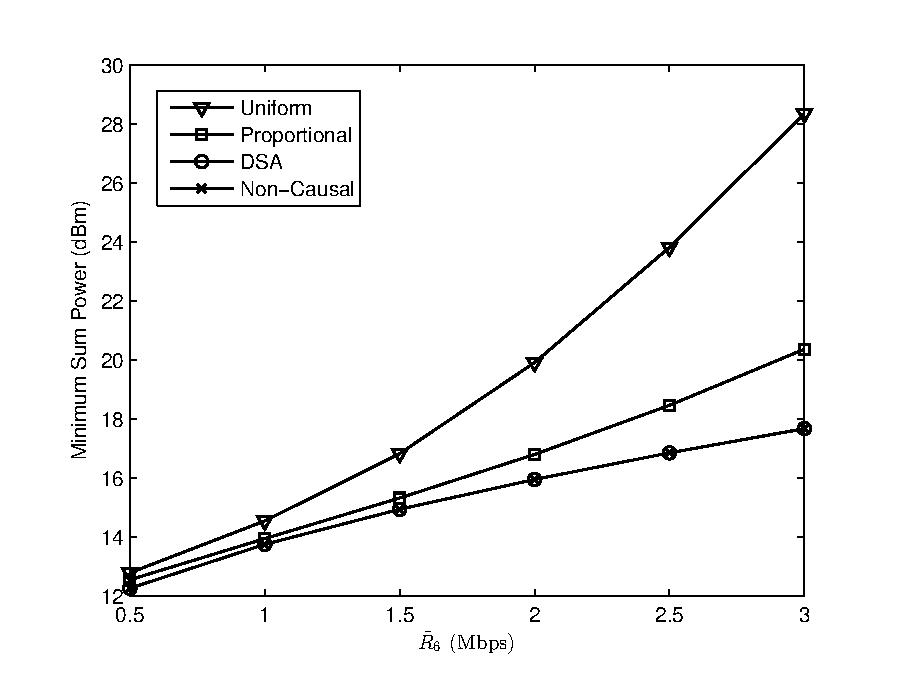
\includegraphics[width=3.6in]{fig2.eps}
\caption{Minimum sum power versus $\bar{R}_6$; comparison of our proposed dynamic spectrum acquisition scheme, the ``Uniform" scheme, the ``Proportional" scheme, and the ``Non-Causal" scheme.}
\end{figure}

In Fig. 3, we present the bandwidth allocation comparison of different schemes when $\bar{R}_6=2$ Mbps. From Fig. 3, it is found that the allocated bandwidth of our proposed dynamic spectrum acquisition scheme is almost the same as that of the ``Non-Causal" scheme.

\begin{figure}
\centering
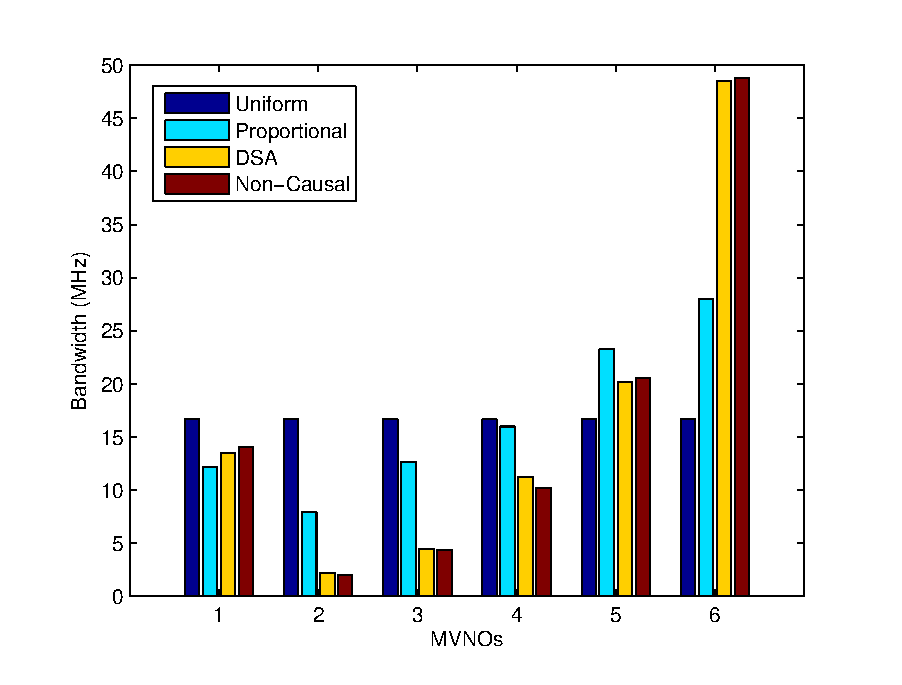
\includegraphics[width=3.6in]{fig3.eps}
\caption{Bandwidth allocation comparison of our proposed dynamic spectrum acquisition scheme, the ``Uniform" scheme, the ``Proportional" scheme, and the ``Non-Causal" scheme when $\bar{R}_6=2$ Mbps.}
\end{figure}

In Fig. 4, we vary the value of $\lambda_6$ while remaining $\lambda_1$, $\lambda_2$, $\cdots$, $\lambda_5$ to be constant and present the minimum sum power comparison of different schemes. In Fig. 5, we present the corresponding bandwidth allocation of our proposed dynamic spectrum acquisition scheme for all MVNOs. From Fig. 4, it is shown that almost the same minimum sum power is obtained by our proposed dynamic spectrum acquisition scheme and the ``Non-Causal" scheme.

\begin{figure}
\centering
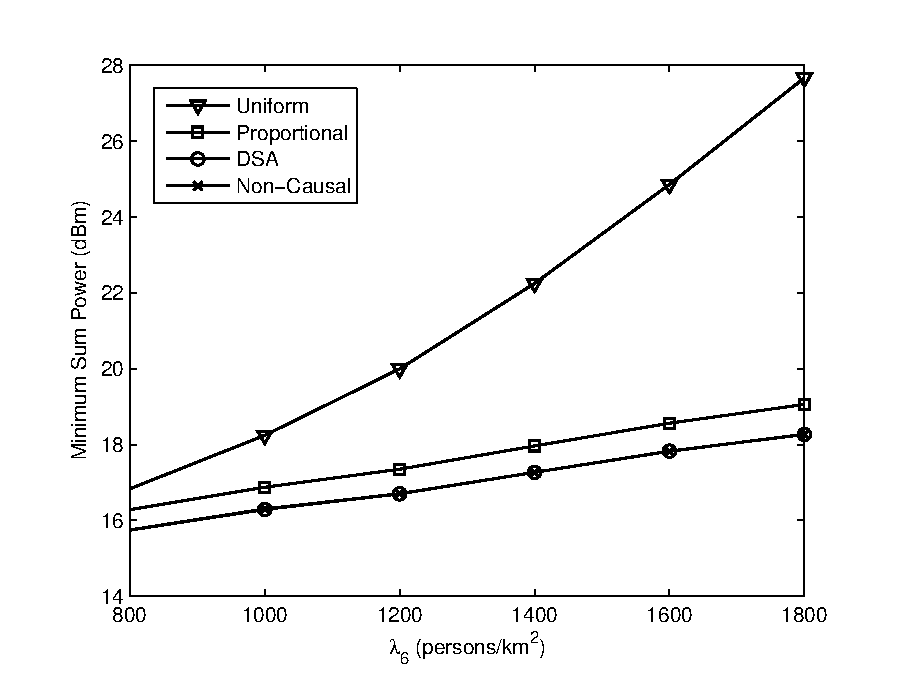
\includegraphics[width=3.6in]{fig4.eps}
\caption{Minimum sum power versus $\lambda_6$; comparison of our proposed dynamic spectrum acquisition scheme, the ``Uniform" scheme, the ``Proportional" scheme, and the ``Non-Causal" scheme when $\bar{R}_1 =\tilde{R}_1=2$ Mbps, $\bar{R}_2 =\tilde{R}_2=0.5$ Mbps, $\bar{R}_3=\tilde{R}_3=0.5$ Mbps, $\bar{R}_4 =\tilde{R}_4=1$ Mbps, $\bar{R}_5=\tilde{R}_5=1$ Mbps, and $\bar{R}_6 =\tilde{R}_6=2$ Mbps.}
\end{figure}

\begin{figure}
\centering
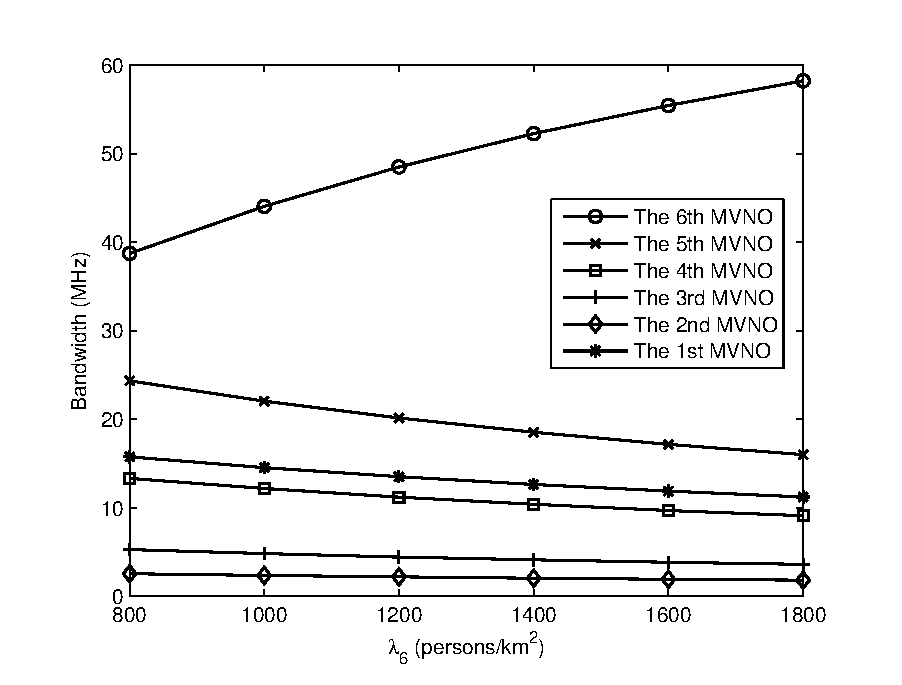
\includegraphics[width=3.6in]{fig5.eps}
\caption{Bandwidth allocation of all MVNOs versus $\lambda_6$; our proposed dynamic spectrum acquisition scheme when $\bar{R}_1 =\tilde{R}_1=2$ Mbps, $\bar{R}_2 =\tilde{R}_2=0.5$ Mbps, $\bar{R}_3=\tilde{R}_3=0.5$ Mbps, $\bar{R}_4 =\tilde{R}_4=1$ Mbps, $\bar{R}_5=\tilde{R}_5=1$ Mbps, and $\bar{R}_6 =\tilde{R}_6=2$ Mbps.}
\end{figure}

\section{Conclusion}
In this paper, we have proposed a decentralized blockchain based dynamic spectrum acquisition scheme for a wireless downlink communication system with multiple MVNOs. It is shown through simulation results that our proposed dynamic spectrum acquisition scheme achieves almost the same minimum sum power as the non-causal scheme which assumes the number of active MUs in all cells and all the channels are known non-causally for optimal dynamic spectrum allocation.

\appendices
\section{Proof of Proposition 1}

According to the definition of the CDF, we have
\begin{align}
F_{\left|h_{mn} \right|^2} \left(x\right)=\mbox{Pr}\left(\left|g_{mn}\right|^2 \leq x \left(1 + L_{mn}^\alpha\right)\right).
\end{align}
Since $g_{mn}$ is a complex Gaussian random variable with zero mean and unit variance,  $\left|g_{ij}\right|^2$ is an exponentially distributed random variable.
Furthermore, the location of the $n$-th MU in the $m$-th cell is uniformly distributed in $\mathcal{D}_m$ with the PDF of $1/(\pi r_m^2)$. By using polar coordinates, we obtain
\begin{align}
F_{\left|h_{mn}\right|^2} \left(x\right)= \int_{0}^{r_m} \int_{-\pi}^{\pi}\frac{1}{\pi r_m^2}\left(1 - e^{-x\left(1 + y^{\alpha}\right)}\right)y d \theta d y.
\end{align}
After some mathematical manipulation, we obtain
\begin{align}
F_{\left|h_{mn}\right|^2} \left(x\right)=1-\frac{2}{r_m^2}e^{-x} \int_{0}^{r_m}y e^{-xy^{\alpha}}dy.
\end{align}
Let $t = xy^{\alpha}$. $F_{\left|h_{mn}\right|^2} \left(x\right)$ is reexpressed as
\begin{align}
F_{\left|h_{mn}\right|^2} \left(x\right) &= 1 - \frac{2}{r_m^2}e^{-x} \int_{0}^{x r_m^{\alpha}} t^{\frac{1}{\alpha}} x^{-\frac{1}{\alpha}}e^{-t} d\left(t^{\frac{1}{\alpha}} x^{-\frac{1}{\alpha}}\right)\nonumber\\
& = 1 - \frac{2}{\alpha r_m^2}x^{-\frac{2}{\alpha}} e^{-x} \int_{0}^{x r_m^{\alpha}} t^{\frac{2}{\alpha} - 1}e^{-t} dt\nonumber\\
& = 1 - \frac{2}{\alpha} \left(x r_m^{\alpha}\right) ^{-\frac{2}{\alpha}} \gamma\left(\frac{2}{\alpha}, x r_m^{\alpha}\right)e^{-x}
\end{align}
where $\gamma\left(s,x\right) = \int_{0}^{x}t^{s-1}e^{-t}dt$ denotes the lower incomplete gamma function. Because $\Psi\left(s,1+s,-x\right)=sx^{-s}\gamma\left(s,x\right)$ \cite[6.5.12]{MAbramowitz}, we obtain \eqref{q9}.

\section{Proof of Proposition 2}

We prove Proposition 2 by contradiction. Assume that $\mathbf{q}_m^\star=[q_{m1}^\star, q_{m2}^\star, \cdots, q_{mN_m}^\star]^T$ is the optimal solution to problem \eqref{cq1} such that there exists $n\in\mathcal{N}_m$ which satisfy
\begin{align}
b_{mn}\log_2\left(1 + \frac{q_{mn}\left|h_{mn}\right|^2}{b_{mn}\sigma^2}\right)>\tilde{R}_m.
\end{align}
We can choose a proper real scalar $\Delta>0$ such that
\begin{align}
b_{mn}\log_2\left(1 + \frac{(q_{mn}^\star-\Delta)\left|h_{mn}\right|^2}{b_{mn}\sigma^2}\right)=\tilde{R}_m.
\end{align}
Note that $[q_{m1}^\star, \cdots, q_{m(n-1)}^\star, q_{mn}^\star-\Delta, q_{m(n+1)}^\star, \cdots, q_{mN_m}^\star]^T$ is also feasible and has smaller objective value than $\mathbf{q}_m^\star$. This contradicts that $\mathbf{q}_m^\star$ is the optimal solution.

\section{Proof of Proposition 3}
The Lagrangian of problem \eqref{cq3} is given by
\begin{align}
\tilde{\mathcal{L}}=&\sum\limits_{n= 1}^{N_m} \frac{b_{mn}\sigma^2}{\left|h_{mn}\right|^2}\left(e^{\frac{\tilde{R}_m\ln2}{b_{mn}}} - 1\right)+\mu\left(\sum_{n= 1}^{N_m}b_{mn} - w_m\right)
\end{align}
where $\mu\geq 0$ denotes the Lagrange multiplier associated with the constraint $\sum_{n=1}^{N_m} b_{mn}\leq w_m$. Since problem \eqref{cq3} is convex, the Karush-Kuhn-Tucker (KKT) conditions are both necessary and 	sufficient for the global optimality of problem \eqref{cq3}. It can be verified that $\sum_{n=1}^{N_m} b_{mn}=w_m$ must hold for problem \eqref{cq1}. From KKT conditions, we have $\mu^o > 0$ where $\mu^o$ denotes the optimal dual solution to problem \eqref{cq3}.

Taking the first-order partial derivative of $\tilde{\mathcal{L}}$ with respect to $b_{mn}$, we have
\begin{equation}
\frac{\partial \tilde{\mathcal{L}}}{\partial b_{mn}}=  \frac{\sigma^2}{\left|h_{mn}\right|^2}\left(\left(1 - \frac{\tilde{R}_m\ln2}{b_{mn}}\right)e^{\frac{\tilde{R}_m\ln2}{b_{mn}}}- 1\right) + \mu
\end{equation}
From KKT conditions, we have
\begin{align}
\left(\frac{\tilde{R}_m\ln2}{b_{mn}^o} - 1\right)e^{\frac{\tilde{R}_m\ln2}{b_{mn}^o}-1}= \frac{\mu^o \left|h_{mn}\right|^2 - \sigma^2}{e\sigma^2}.
\end{align}
According to the definition of Lambert $\mathcal{W}$ function, we obtain the optimal $b_{mn}^o$ as in \eqref{cq4}. In \eqref{cq4}, there exists an unknown parameter $\mu^o$. The value of $\mu^o$ should satisfy $\sum_{n=1}^{N_m} b_{mn}=w_m$.

In \eqref{cq4}, since
\begin{equation}
\frac{\mu^o\left|h_{mn}\right|^2 - \sigma^2}{e\sigma^2}\geq-1,
\end{equation}
$\mathcal{W}\left(x\right)$ is a monotonically increasing function. Accordingly, $b_{mn}^o$ is a monotonically decreasing function of $\left|h_{mn}\right|^2$. Thus, we have
\begin{align}\label{dq4}
&\frac{\tilde{R}_m\ln2}{1 + \mathcal{W}\left(\frac{\mu^o\max_n\left|h_{mn}\right|^2 - \sigma^2}{e\sigma^2}\right)}\leq b_{mn}^o \nonumber\\ &\leq  \frac{\tilde{R}_m\ln2}{1 + \mathcal{W}\left(\frac{\mu^o\min_n\left|h_{mn}\right|^2 - \sigma^2}{e\sigma^2}\right)}
\end{align}
Summing each term in \eqref{dq4} from $n=1$ to $n= N_m$, we obtain
\begin{align}
&\frac{N_m\tilde{R}_m\ln2}{1 + \mathcal{W}\left(\frac{\mu^o\max_n\left|h_{mn}\right|^2 - \sigma^2}{e\sigma^2}\right)}\leq w_{m} \nonumber\\ &\leq  \frac{N_m\tilde{R}_m\ln2}{1 + \mathcal{W}\left(\frac{\mu^o\min_n\left|h_{mn}\right|^2 - \sigma^2}{e\sigma^2}\right)}
\end{align}
According to the definition of Lambert $\mathcal{W}$ function, we have
\begin{align}
\mu_{\min} \leq \mu^o \leq \mu_{\max}
\end{align}
where $\mu_{\min}$ and $\mu_{\max}$ are defined in \eqref{cq5}.

\begin{thebibliography}{1}	
\bibitem{NPanwar} N. Panwar, S. Sharma, and A. K. Singh, ``A survey on 5G: The next generation of mobile communication," \emph{Phys. Commun.}, vol. 18, pp. 64-84, Mar. 2016.

\bibitem{DingZ14} Z. Ding, Z. Yang, P. Fan, and H. V. Poor, ``On the performance of nonorthogonal multiple access in 5G systems with randomly deployed users," \emph{IEEE Signal Process. Lett.}, vol. 21, no. 12, pp. 1501-1505, Dec. 2014.

\bibitem{LiY17} Y. Li, M. Jiang, Q. Zhang, Q. Li, and J. Qin, ``Secure beamforming in downlink MISO nonorthogonal multiple access systems," \emph{IEEE Trans. Veh. Technol.}, vol. 66, no. 8, pp. 7563-7567, Aug. 2017.

\bibitem{LiY18} Y. Li, M. Jiang, Q. Zhang, Q. Li, and J. Qin, ``Cooperative non-orthogonal multiple access in multiple-input-multiple-output channels," \emph{IEEE Trans. Wireless Commun.}, vol. 17, no. 3, pp. 2068-2079, Mar. 2018.

\bibitem{AYDing} A. Y. Ding and M. Janssen, ``Opportunities for applications using 5G networks: Requirements, challenges, and outlook," in \emph{Proc. of International Conference on Telecommunications and Remote Sensing, 2018}, pp. 27-34.
	
\bibitem{CLiang} C. Liang and F. R. Yu, ``Wireless network virtualization: A survey, some research issues and challenges," \emph{IEEE Comm. Surveys Tuts.}, vol. 17, no. 1, pp. 358-380, First Quart. 2015.

\bibitem{LZhao} L. Zhao, M. Li, Y. Zaki, A. Timm-Giel, and C. G\"org, ``LTE virtualization: From theoretical gain to practical solution," in \emph{Proc. International Teletraffic Congress, 2011}, pp. 71-78.

\bibitem{3GPP} 3GPP TR 22.852, ``Study on radio access network (RAN) sharing enhancements," Jun. 2013.

\bibitem{RKokku} R. Kokku, R. Mahindra, H. Zhang, and S. Rangarajan, ``NVS: A substrate for virtualizing wireless resources in cellular networks," \emph{IEEE/ACM Trans. Netw.}, vol. 20, no. 5, pp. 1333-1346, Oct. 2012.

\bibitem{XCostaPerez} X. Costa-Perez, J. Swetina, T. Guo, R. Mahindra, and S. Rangarajan, ``Radio access network virtualization for future mobile carrier networks," \emph{IEEE Commun. Mag.}, vol. 51, no. 7, pp. 27-35, Jul. 2013.

\bibitem{MIKamel} M. I. Kamel, L. B. Le, and A. Girard, ``LTE wireless network virtualization: Dynamic slicing via flexible scheduling," in \emph{Proc. IEEE VTC, 2014}, pp. 1-5.

\bibitem{MKalil} M. Kalil, A. Moubayed, A. Shami, and A. Al-Dweik, ``Efficient low-complexity scheduler for wireless resource virtualization," \emph{IEEE Wireless Commun. Lett.}, vol. 5, no. 1, pp. 56-59, Feb. 2016.
	
\bibitem{YXZhang} Y. Zhang, S. Bi, and Y. J. A. Zhang, ``Joint spectrum reservation and on-demand request for mobile virtual network operators," \emph{IEEE Trans. Commun.}, vol. 66, no. 7, pp. 2966-2977, Jul. 2018.

\bibitem{SNakamoto} S. Nakamoto, ``Bitcoin: A peer-to-peer electronic cash system," 2008. [Online]. Available: https://bitcoin.org/bitcoin.pdf

\bibitem{KGai} K. Gai, K.-K. R. Choo, and L. Zhu, ``Blockchain-enabled reengineering of cloud datacenters," \emph{IEEE Cloud Comput.}, vol. 5, no. 6, pp. 21-25, Nov. 2018.

\bibitem{PKSharma} P. K. Sharma, S. Singh, Y. S. Jeong, and J. H. Park, ``DistBlockNet: A distributed blockchains-based secure SDN architecture for IoT networks," \emph{IEEE Commun. Mag.}, vol. 55, no. 9, pp. 78-85, Sept. 2017.

\bibitem{ZXiong} Z. Xiong, S. Feng, W. Wang, D. Niyato, P. Wang, and Z. Han, ``Cloud/fog computing resource management and pricing for blockchain networks," \emph{IEEE Internet Things J.}, to be published.

\bibitem{DBRawat} D. B. Rawat and A. Alshaikhi, ``Leveraging distributed blockchain-based scheme for wireless network virtualization with security and QoS constraints," in \emph{Proc. International Conference on Computing, Networking and Communications, 2018}, pp. 332-336.

\bibitem{Munsing} E. M\"{u}nsing, J. Mather, and S. Moura, ``Blockchains for decentralized optimization of energy resources in microgrid networks," in \emph{Proc. IEEE Conference on Control Technology and Applications, 2017}, pp. 2164-2171.

\bibitem{KKotobi} K. Kotobi and S. G. Bilen, ``Secure blockchains for dynamic spectrum access: A decentralized database in moving cognitive radio networks enhances security and user access," \emph{IEEE Veh. Technol. Mag.}, vol. 13, no. 1, pp. 32-39, Mar. 2018.
	
\bibitem{JGDForney} J. G. D. Forney and G. Ungerboeck, ``Modulation and coding for linear Gaussian channels," \emph{IEEE Trans. Inf. Theory}, vol. 44, no. 6, pp. 2384-2415, Oct. 1998.

\bibitem{MAbramowitz} M. Abramowitz and I. A. Stegun, \emph{Handbook of Mathematical Functions with Formulas, Graphs, and Mathematical Tables}. New York, NY, USA: Dover, 1972.

\bibitem{JSBall} J. S. Ball, ``Half-range generalized Hermite polynomials and the related Gaussian quadratures," \emph{SIAM J. Numer. Anal.}, vol. 40, no. 6, pp. 2311-2317, 2002.

\bibitem{NMSteen} N. M. Steen, G. D. Byrne, and E. M. Gelbard, ``Gaussian quadratures for the integrals $\int_{0}^{\infty} e^{-x^2}f\left(x\right) dx$ and $\int_{0}^{b}e^{-x^2}f\left(x\right)dx$," \emph{Math. Comput.}, vol. 23, no. 107, pp. 661-671, 1969.

\bibitem{SBoyd1} S. Boyd and L. Vandenberghe, \emph{Convex Optimization}. Cambridge, U.K.: Cambridge Univ. Press, 2004.

\bibitem{SBoyd2} S. Boyd, N. Parikh, E. Chu, B. Peleato, and J. Eckstein, ``Distributed optimization and statistical learning via the alternating direction method of multipliers," \emph{Found. Trends in Mach. Learn.}, vol. 3, no. 1, pp. 1-122, Jan. 2011.

\bibitem{EChen} E. Chen and M. Tao, ``ADMM-based fast algorithm for multi-group multicast beamforming in large-scale wireless systems," \emph{IEEE Trans. Commun.}, vol. 65, no. 6, pp. 2685-2698, Jun. 2017.

\bibitem{JDuchi} J. Duchi, S. Shalev-Shwartz, Y. Singer, and T. Chandra, ``Efficient projections onto the $l_1$-ball for learning in high dimensions," in \emph{Proc. International Conference on Machine Learning, 2008}.

\bibitem{RMCorless} R. M. Corless, G. H. Gonnet, D. E. G. Hare, D. J. Jeffrey, and D. E. Knuth, ``On the Lambert W function," \emph{Adv. Comput. Math.}, vol. 5, pp. 329-359, 1996.

\bibitem{3GPP2} 3GPP TR 36.931, ``LTE; evolved universal terrestrial radio access (E-UTRA); radio frequency (RF) requirements for LTE pico Node B,"
    May 2011.

\end{thebibliography}


\end{document}
